\section{VALIDATION}
\label{sec:validation}

\subsection{On bearings vibration datasets}

The PC implementation of the framework has been thoroughly tested on a publicly available dataset provided by the Center for Intelligent Maintenance Systems (IMS).
%\footnote{\url{https://www.nasa.gov/intelligent-systems-division/discovery-and-systems-health/pcoe/pcoe-data-set-repository/}}
The dataset contains time series of the vibration of four bearings, for a total of three separate \quoted{run to failure} experiences. The dataset provides information about the location and type of defects observed after each test.

\begin{figure}
    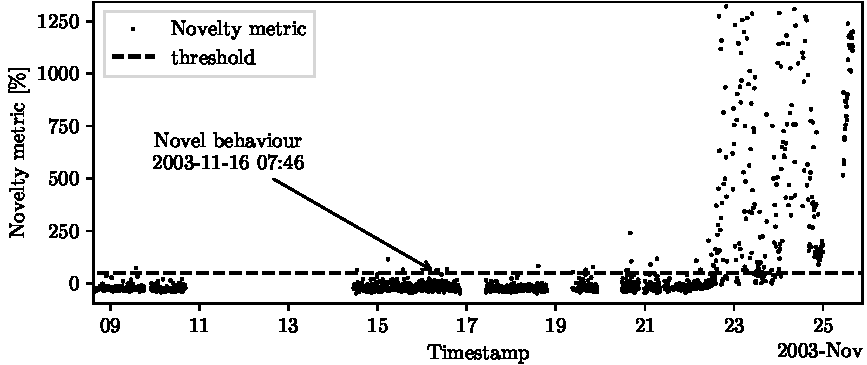
\includegraphics[width=\linewidth]{images/ND_IMS.pdf}
    \caption{Results of ND on the IMS dataset}
    \label{fig:ND_IMS}
\end{figure}
\begin{table}
    \centering
    \caption{Comparison of the results for the test n$^\circ$1 of IMS dataset.}
    \label{tab:ims01_comparision}
    \begin{tabular}{lcrr} 
    \toprule
    \textbf{Algorithm} & \textbf{ND event} & \textbf{LT }{[}min] & \textbf{LT }{[}days] \\ 
    \hline
    K-means & 2003-11-16 07:46 & \textbf{13913} & \textbf{9.6} \\
    DBSCAN & 2003-11-22 15:06 & 4833 & 3.3\\
    GMM & 2003-11-22 03:47 & 5513 & 3.8\\
    BGMM & 2003-11-22 03:45 & 5514 & 3.8\\
    $\nu$-SVM & 2003-11-22 14:56 & 4844 &3.3\\
    IF & 2003-11-16 10:08 & 13771 & 9.6\\
    LOF & 2003-11-16 07:48 & 13912 & 9.6\\
    {P2P} without any ML & 2003-11-22 16:06 & 4774 & 3.3\\
    \bottomrule
    \end{tabular}
\end{table}
The ND capability of the framework has been tested using all the UML models. The lead time (LT) elapsed between the ND event and the actual fault is used to compare the models. The results are compared in table~\ref{tab:ims01_comparision}. The evolution of the NM, using a K-means model on the "Bearing 3x" signal of the test N$^\circ$1, is shown in Fig.~\ref{fig:ND_IMS}.

\begin{figure}
    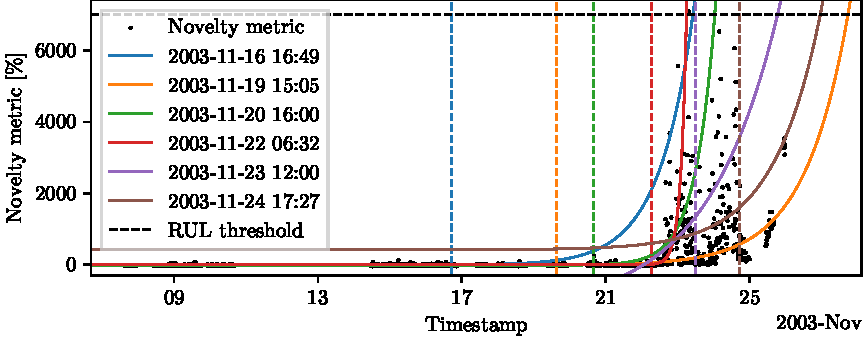
\includegraphics[width=\linewidth]{images/RUL_IMS.pdf}
    \caption{Results of RUL predictions on the IMS dataset}
    \label{fig:RUL_IMS}
\end{figure}
To perform PM, the framework has to estimate the Remaining Useful Life (RUL) of the system. The RUL is predicted computing when a fitted curve crosses a certain threshold. The type of curve to fit is configurable, in this work $y = a \cdot e^{b \cdot x} + c$ has been used. The results of the RUL predictions are shown in Fig.~\ref{fig:RUL_IMS}.

\begin{figure}
    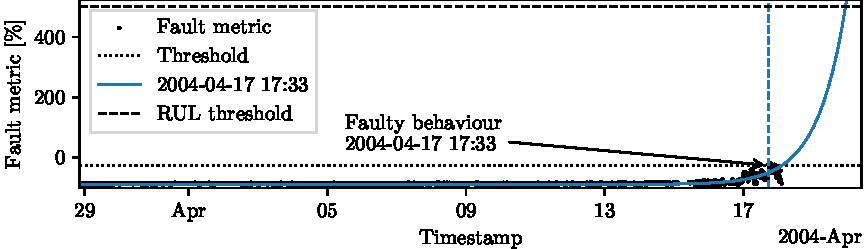
\includegraphics[width=\linewidth]{images/FD_IMS.pdf}
    \caption{Results of FD on the IMS dataset}
    \label{fig:FD_IMS}
\end{figure}
Since the second and third tests of the IMS dataset share the same kind of fault, the framework has been trained to perform FD with the faulty data of the second test and then evaluated on the third. Analogously to the ND, after the FM crosses a certain threshold, a warning is issued and RUL predictions are performed. The results of the FD are shown in Fig.~\ref{fig:FD_IMS}.

\subsection{Laboratory tests}

\begin{figure}
    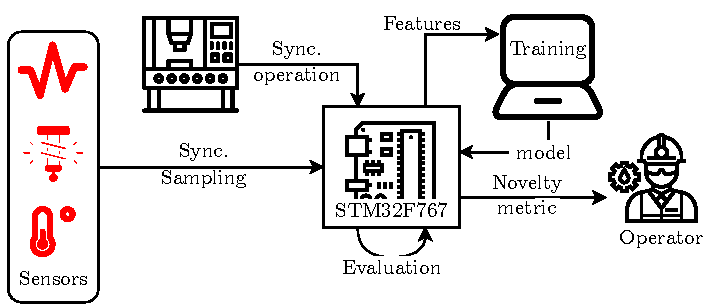
\includegraphics[width=\linewidth]{images/EmbeddedStructure.pdf}
    \caption{Structure of the Edge implementation}
    \label{fig:embedded}
\end{figure}

Since the validation on the IMS dataset has shown that the K-means model is both the simplest and the most effective, it has been deployed on the Edge implementation. In the first phase, the framework gathers the data, extracts the features and sends them to a PC. The UML model is trained on the PC and then sent back to the Edge. After, the microcontroller autonomously evaluates the status of the maintained system. The structure of the Edge implementation is shown in Fig.~\ref{fig:embedded}.

\begin{figure}
    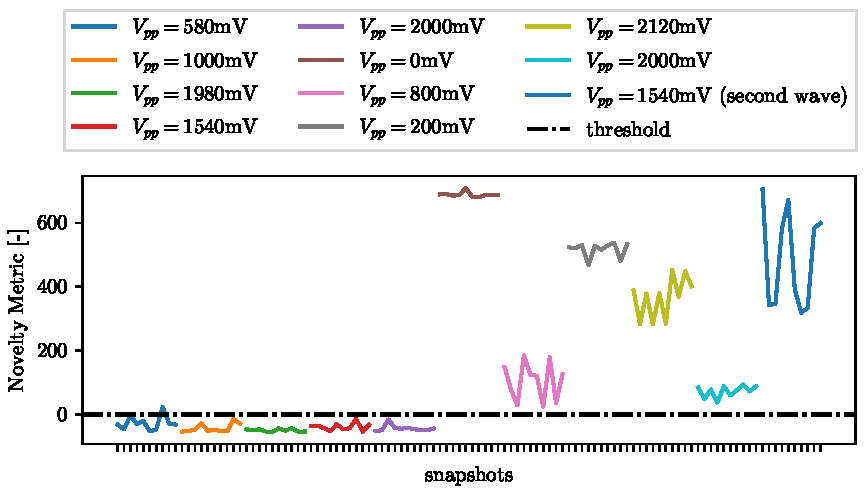
\includegraphics[width=\linewidth]{images/Test02_LOF.pdf}
    \caption{Results of laboratory test on shaker vibrations}
    \label{fig:shaker}
\end{figure}

Extensive tests have been performed on a laboratory shaker, simulating the vibrations generated by a generic mechanical system. The tests have been carried out to evaluate the sensitivity to variations in both amplitude and frequency content of the vibrations. In Fig.~\ref{fig:shaker} the results of the ND are shown. The first five lines are novelty evaluations a repetition of the same signals used for training, and the remaining lines are the successful detections of the novelty.

A second series of tests has been performed mounting the accelerometer on a linear actuator. The axis of the accelerometer has been aligned with the direction of the movement of the actuator, to sense more the acceleration actuated rather than the vibrations. A set of predefined movement profiles has been used for training, while another set for testing. This series of tests exploited a high number of non-significant features. This is because the WPD gave high resolution on a wide range of frequency content, but the actuator excited only a few, and very low, frequencies. The remaining features were almost all noise, and the standardization procedure had the side effect of amplifying them to the same level as the significant ones. An effort has been made to fine-tune the model to reduce the impact of the noise (see Fig.~\ref{fig:linear}, models 1 to 4). The best result, however, has been obtained by removing the less informative features and using a reduced feature space. The benefit of this approach is evident in Fig.~\ref{fig:linear}, as \quoted{Model 5} shows a clear and sharp detection of the alternating pattern between known and unknown movement profiles.


\begin{figure}
    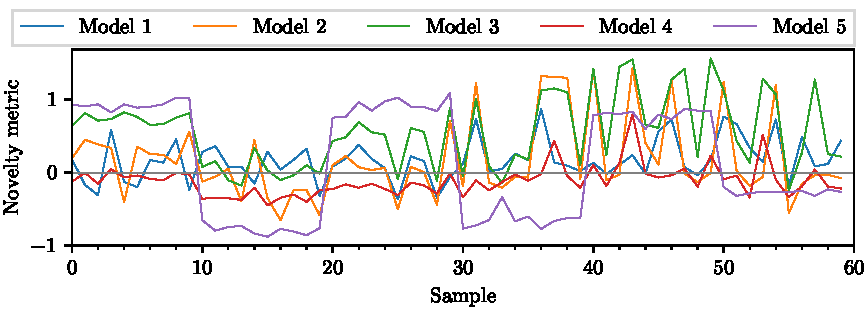
\includegraphics[width=\linewidth]{images/linear.pdf}
    \caption{Results of laboratory test on linear actuator acceleration profiles}
    \label{fig:linear}
\end{figure}